\section{Phương Pháp Đề Xuất}
\label{sec:method}

\subsection{Hai Footprint Phân Giải Vật Lý}
Xét một câu hỏi $q$ liên quan đến đối tượng thuộc lớp địa vật $c$ trong ảnh viễn thám $I$ có độ phân giải không gian danh định (GSD) là $\gsd$ (mét/pixel). Gọi $L$ (mét) là kích thước vật lý đặc trưng của đối tượng:
\begin{itemize}
    \item Nếu câu hỏi truy vấn một thực thể cụ thể có bounding box hoặc polygon, $L = \min(w, h) \cdot \gsd$, tức chiều nhỏ nhất của đối tượng trên thực địa.
    \item Nếu câu hỏi truy vấn sự tồn tại của một lớp đối tượng tổng quát (chưa biết có trong ảnh hay không), $L = L_c^{\min}$ - kích thước tối thiểu hợp lý theo tiêu chuẩn vật lý của lớp $c$ (được tra cứu từ bảng thông số phương tiện và công trình chuẩn hóa quốc tế).
\end{itemize}

\textit{Footprint theo pixel cảm biến} ($\rhopx$): Được định nghĩa là số pixel vật lý trên chiều nhỏ của vật thể mà cảm biến vệ tinh ghi nhận:
\begin{equation}
\rhopx = \frac{L}{\gsd}.
\label{eq:rhopx}
\end{equation}
Đại lượng $\rhopx$ hoàn toàn độc lập với mô hình thị giác và phản ánh năng lực thu nhận nguyên bản của phần cứng cảm biến (tương ứng với đại lượng số chu kỳ tới hạn trong tiêu chí Johnson).

\textit{Footprint theo token bộ mã hóa} ($\rhotok$): Khi ảnh viễn thám $I$ được đưa vào mô hình MLLM $m$, bộ tiền xử lý hình ảnh sẽ thực hiện co giãn, chia lưới (\textit{tiling}) hoặc lấy mẫu lại với hệ số tỷ lệ $s_m(I)$. Sau đó, ảnh được chia thành các patch có kích thước cơ sở $p$ và gộp qua các lớp gộp token (\textit{MLP merger} hoặc \textit{pixel unshuffle}) tạo thành patch hiệu dụng $P_m$ (pixel mô hình trên mỗi token biểu diễn). Footprint theo token trên view thuận lợi nhất chứa đối tượng được định nghĩa là:
\begin{equation}
\rhotok^{(m)}(q, I) = \max_{v \ni \text{obj}} \rhopx \cdot \frac{s_m(I, v)}{P_m}.
\label{eq:rhotok}
\end{equation}

\begin{table}[t]
\centering
\caption{Bộ mã hóa thị giác, patch hiệu dụng $P$ và chính sách phân giải của 5 mô hình RS-MLLM trong nghiên cứu.}
\label{tab:models_arch}
\resizebox{\columnwidth}{!}{%
\begin{tabular}{llccc}
\toprule
Mô hình & Bộ mã hóa thị giác & Patch $p$ & Gộp token & Patch hiệu dụng $P$ \\
\midrule
GeoChat-7B \cite{geochat2024} & CLIP-ViT-L/14@504 & 14 px & Không & 14 px/token \\
LLaVA-1.5-7B \cite{llava15} & CLIP-ViT-L/14@336 & 14 px & Không & 14 px/token \\
LLaVA-NeXT-7B \cite{llavanext2024} & CLIP-ViT-L/14 AnyRes & 14 px & Không & 14 px/token \\
InternVL3.5-8B \cite{internvl2025} & InternViT-6B (Tile 448) & 14 px & Unshuffle 2x2 & 28 px/token \\
Qwen3-VL-8B \cite{qwen2025vl} & SigLIP2-SO400M (Dynamic) & 16 px & 2D Merger 2x2 & 32 px/token \\
\bottomrule
\end{tabular}%
}
\end{table}

\subsection{Ma Trận 4 Vùng Phân Giải}
Sự kết hợp giữa $\rhopx$ và $\rhotok$ chia không gian bài toán thành 4 vùng phân giải có đặc tính vật lý hoàn toàn khác biệt (Hình~\ref{fig:regimes}):
\begin{enumerate}
    \item \textit{Vùng giới hạn pixel (Pixel-limited)}: $\rhopx < \pzerou$. Thông tin bị thiếu hụt ngay từ bước chụp ảnh của vệ tinh. Mọi cơ chế phóng đại (zoom) hay nội suy chỉ làm tăng kích thước pixel rỗng, không thể khôi phục tín hiệu thực tế. Mô hình bắt buộc phải từ chối (\textit{Abstain}).
    \item \textit{Vùng giới hạn token (Token-limited)}: $\rhopx \ge \pzerou$ nhưng $\rhotok < \rhotokstar$. Thông tin có mặt đầy đủ trên ảnh gốc nhưng bị suy hao do bộ mã hóa ViT nén ảnh vào lưới patch quá lớn. Vùng này là đối tượng duy nhất mà thao tác phóng đại thích nghi (\textit{Zoom}) phát huy tác dụng.
    \item \textit{Vùng phân giải an toàn (Resolvable)}: $\rhopx \ge \pzerou$ và $\rhotok \ge \rhotokstar$. Đối tượng đủ độ phân giải trên cả cảm biến và không gian token; mô hình có thể trả lời trực tiếp với độ tin cậy cao.
    \item \textit{Vùng phóng đại quá mức (Over-tokenized)}: $\rhopx < \pzerou$ nhưng $\rhotok \ge \rhotokstar$ (do ảnh gốc bị phóng to kỹ thuật số trước khi nạp vào mô hình). Vùng này gây ảo giác cao nhất vì mô hình ngộ nhận kích thước pixel kỹ thuật số là chi tiết thực tế.
\end{enumerate}

\begin{figure}[t]
\centering
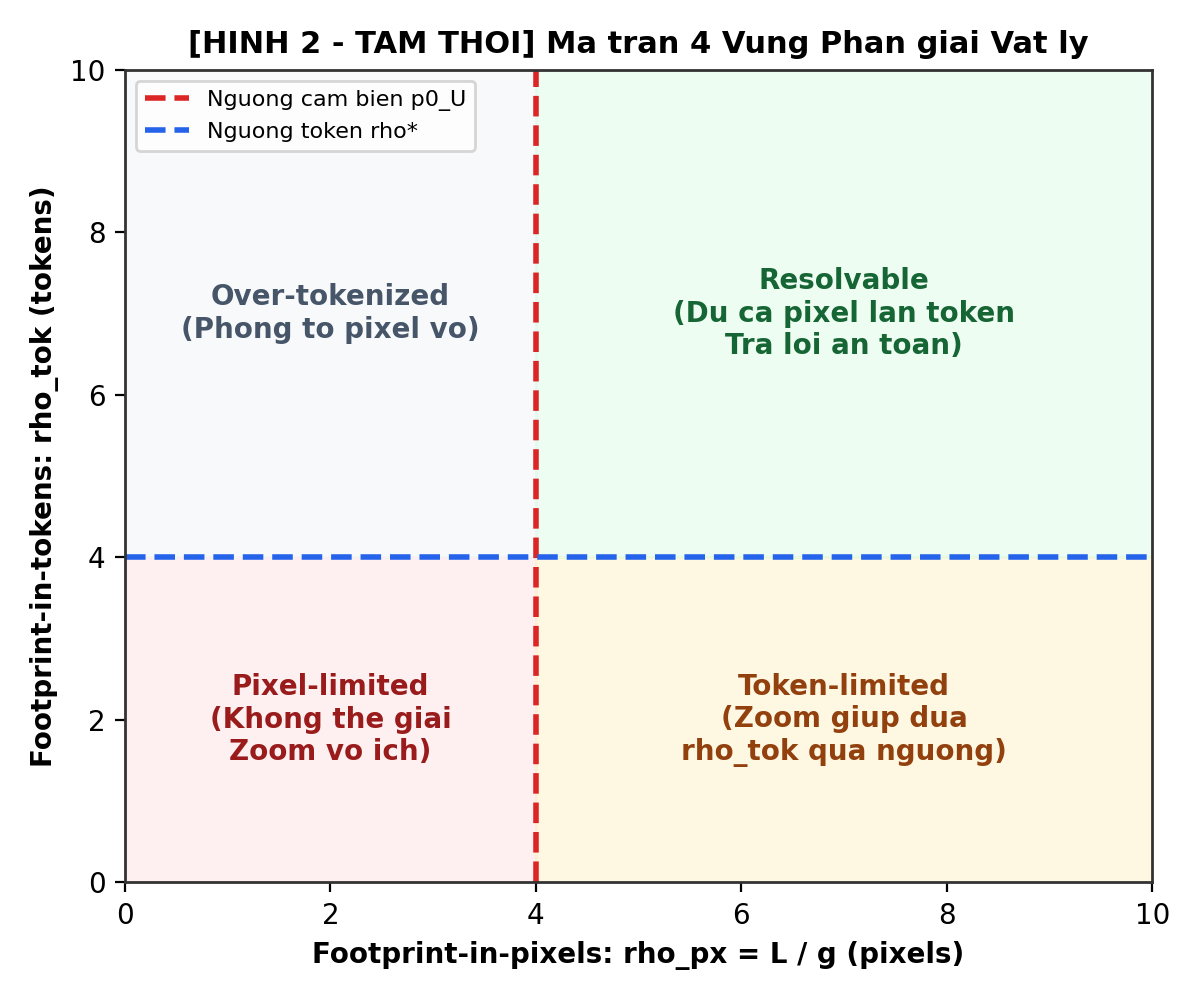
\includegraphics[width=0.85\columnwidth]{figures/fig2_matrix_regimes.png}
\caption{Ma trận 4 vùng phân giải vật lý dựa trên không gian hai chiều $(\rhopx, \rhotok)$.}
\label{fig:regimes}
\end{figure}

\subsection{Bộ Định Tuyến RGSP 4 Nhánh}
Dựa trên ma trận phân giải, chúng tôi thiết kế thuật toán bộ định tuyến RGSP không cần huấn luyện, vận hành hoàn toàn dựa trên các ngưỡng vật lý trước khi chạy mô hình (Thuật toán~\ref{alg:rgsp}).

\begin{algorithm}[t]
\caption{Bộ Định Tuyến RGSP (\textit{Resolvability-Gated Router})}
\label{alg:rgsp}
\begin{algorithmic}[1]
\REQUIRE Ảnh $I$, GSD $\gsd$, Câu hỏi $q$, Kích thước vật lý $L$, Ngưỡng cảm biến $\pzerou$, Ngưỡng token $\rhotokstar$, Hệ số phóng tối đa $s_{\max}$.
\STATE Tính toán $\rhopx = L / \gsd$.
\STATE Tính toán $\rhotok = \rhopx \cdot \frac{s_m(I)}{P_m}$.
\IF{$\rhopx < \pzerou$}
    \STATE return Abstain (``Không thể xác định do giới hạn cảm biến'')
\ENDIF
\STATE Tính toán footprint tối đa khi zoom hết cỡ: $\rhotok^{\max} = \rhopx \cdot \frac{s_{\max}}{P_m}$.
\IF{$\rhotok^{\max} < \rhotokstar$}
    \STATE return Abstain (``Không thể xác định do zoom tối đa không đủ'')
\ELSIF{$\rhotok < \rhotokstar \le \rhotok^{\max}$}
    \STATE Xác định kích thước crop tối ưu: $c^* = \min(w_I, h_I) \cdot \frac{\rhotok}{\rhotokstar}$.
    \STATE Cắt vùng ảnh $I_{\text{crop}}$ kích cỡ $c^*$ quanh đối tượng.
    \STATE return Zoom-and-Answer ($m(I_{\text{crop}}, q)$)
\ELSE
    \STATE return Direct-Answer ($m(I, q)$)
\ENDIF
\end{algorithmic}
\end{algorithm}

\subsection{Hiệu Chỉnh Ngưỡng Bảo Đảm Rủi Ro}
Để đảm bảo rủi ro lựa chọn trên tập chấp nhận trả lời không vượt quá ngưỡng sai số $\alpha$ (ví dụ $\alpha = 10\%$), chúng tôi áp dụng quy trình kiểm định chuỗi cố định (\textit{fixed-sequence testing}) trên tập hiệu chuẩn (\textit{calibration set}):
\begin{equation}
R(\tau) = \frac{\sum_{i=1}^n \mathbb{I}(m(I_i, q_i) \neq y_i) \cdot \mathbb{I}(\rhotok(i) \ge \tau)}{\sum_{i=1}^n \mathbb{I}(\rhotok(i) \ge \tau)}.
\end{equation}
Ngưỡng tối ưu $\tau^*$ được chọn là giá trị nhỏ nhất thỏa mãn cận trên Clopper-Pearson của rủi ro nhỏ hơn $\alpha$ với độ tin cậy $1 - \delta \ge 95\%$.
